\section{Climbing around Camp}

\subsection{\protect\passage{Primula}}

\margininbox{Primula}{
     \begin{itemize}
    \item James Kirkpatrick
    \item Izi Možir
    \end{itemize}}{\explo}


\begin{pagesurvey}
\centering
\frame{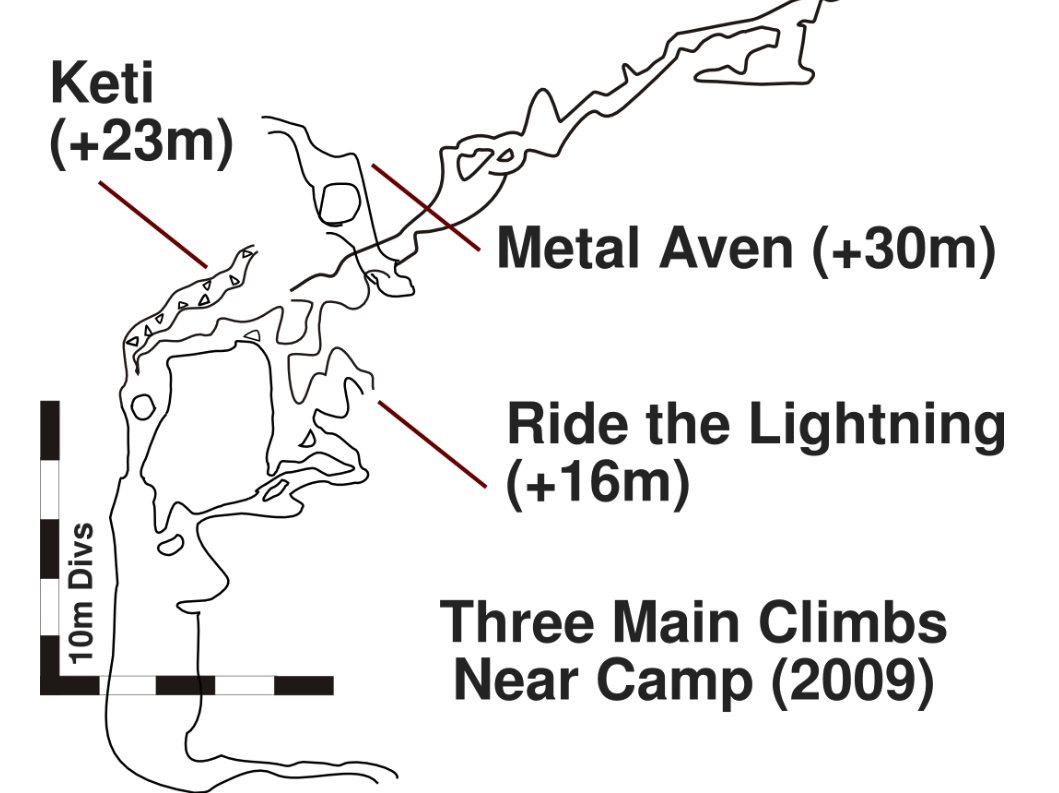
\includegraphics[width=\linewidth]{2009/survey/Screenshot 2023-10-29 at 22-58-47 Slide 1 - BCRA 2009 - Jarvist Frost.pdf.png}}
\caption[2009 \passage{Metal Camp} climbs]{The three climbs around \passage{Metal Camp} that were explored and surveyed in 2009: \passage{Metal Aven}, \passage{K.E.T.I} and \passage{Ride the Lightning}.} \label{camp climbs}
\end{pagesurvey}

James KP and I decided to go camping to \passage{Metal Camp}. I was really
excited to return back to \passage{Captain Kangaroo}, as I have been going
down there for the last 2 years. We quickly arrived to the camp, where
Dan and Jana were resting. We repacked and took what we needed for our
climb. Our plan was to go and push above \passage{Primula}.

At the first rebelay in \passage{Kill 'Em All} pitch, you take the rope up
which leads through meander and then there is a pitch. We descended to
the first ledge, not far down. Here we wanted to make a traverse to the
boulder choke. First we try it with a drill, but it didn't work. Secondly
we try hand bolting it. But because the rock was so bad, we on the end
decided to put a couple of slings around some naturals, to secure James
for the climb. When he reached the boulder choke he quickly put in one
bolt, as \bignote{he did not trust the boulders} above him. After couple of hours
trying to climb through, we then gave up and returned to camp. There
James prepared some food. Don't ask me what we eat, as far as I remember
he boiled some water and then throw in whatever he could find.

\name{Izi Možir}


\subsection{05.08.09 - \protect\passage{Metal Aven}}

\margininbox{Metal Aven}{
     \begin{itemize}
    \item James Kirkpatrick
    \item Izi Možir
    \end{itemize}}{\explo}

When we woke up we felt a bit lazy, so we were wondering what to do; go
out or push a bit more. A plan was made to climb here, directly above
the tent. First 20 m I manage to free climb it; in the meanwhile James
went for the rope. When he returned, he throws me the rope and I secured
it around a big boulder. After that he came up and joined me. The last
10 m was James's turn to climb. Again we secured the rope with couple of
slings around some naturals in case of a fall and James made it to the
top. There he put in some bolts. On the top there was a tunnel, which we
crolled for a while, but then decided it is time to go back and survey.
We named this climb \passage{Metal aven}. After entering data into the
Survex, we discovered that looks like the tunnel is leading to \passage{Dangermouse} pitch, which is just before the camp.

\name{Izi Možir}



\begin{figure*}
\checkoddpage \ifoddpage \forcerectofloat \else \forceversofloat \fi
\centering
 \frame{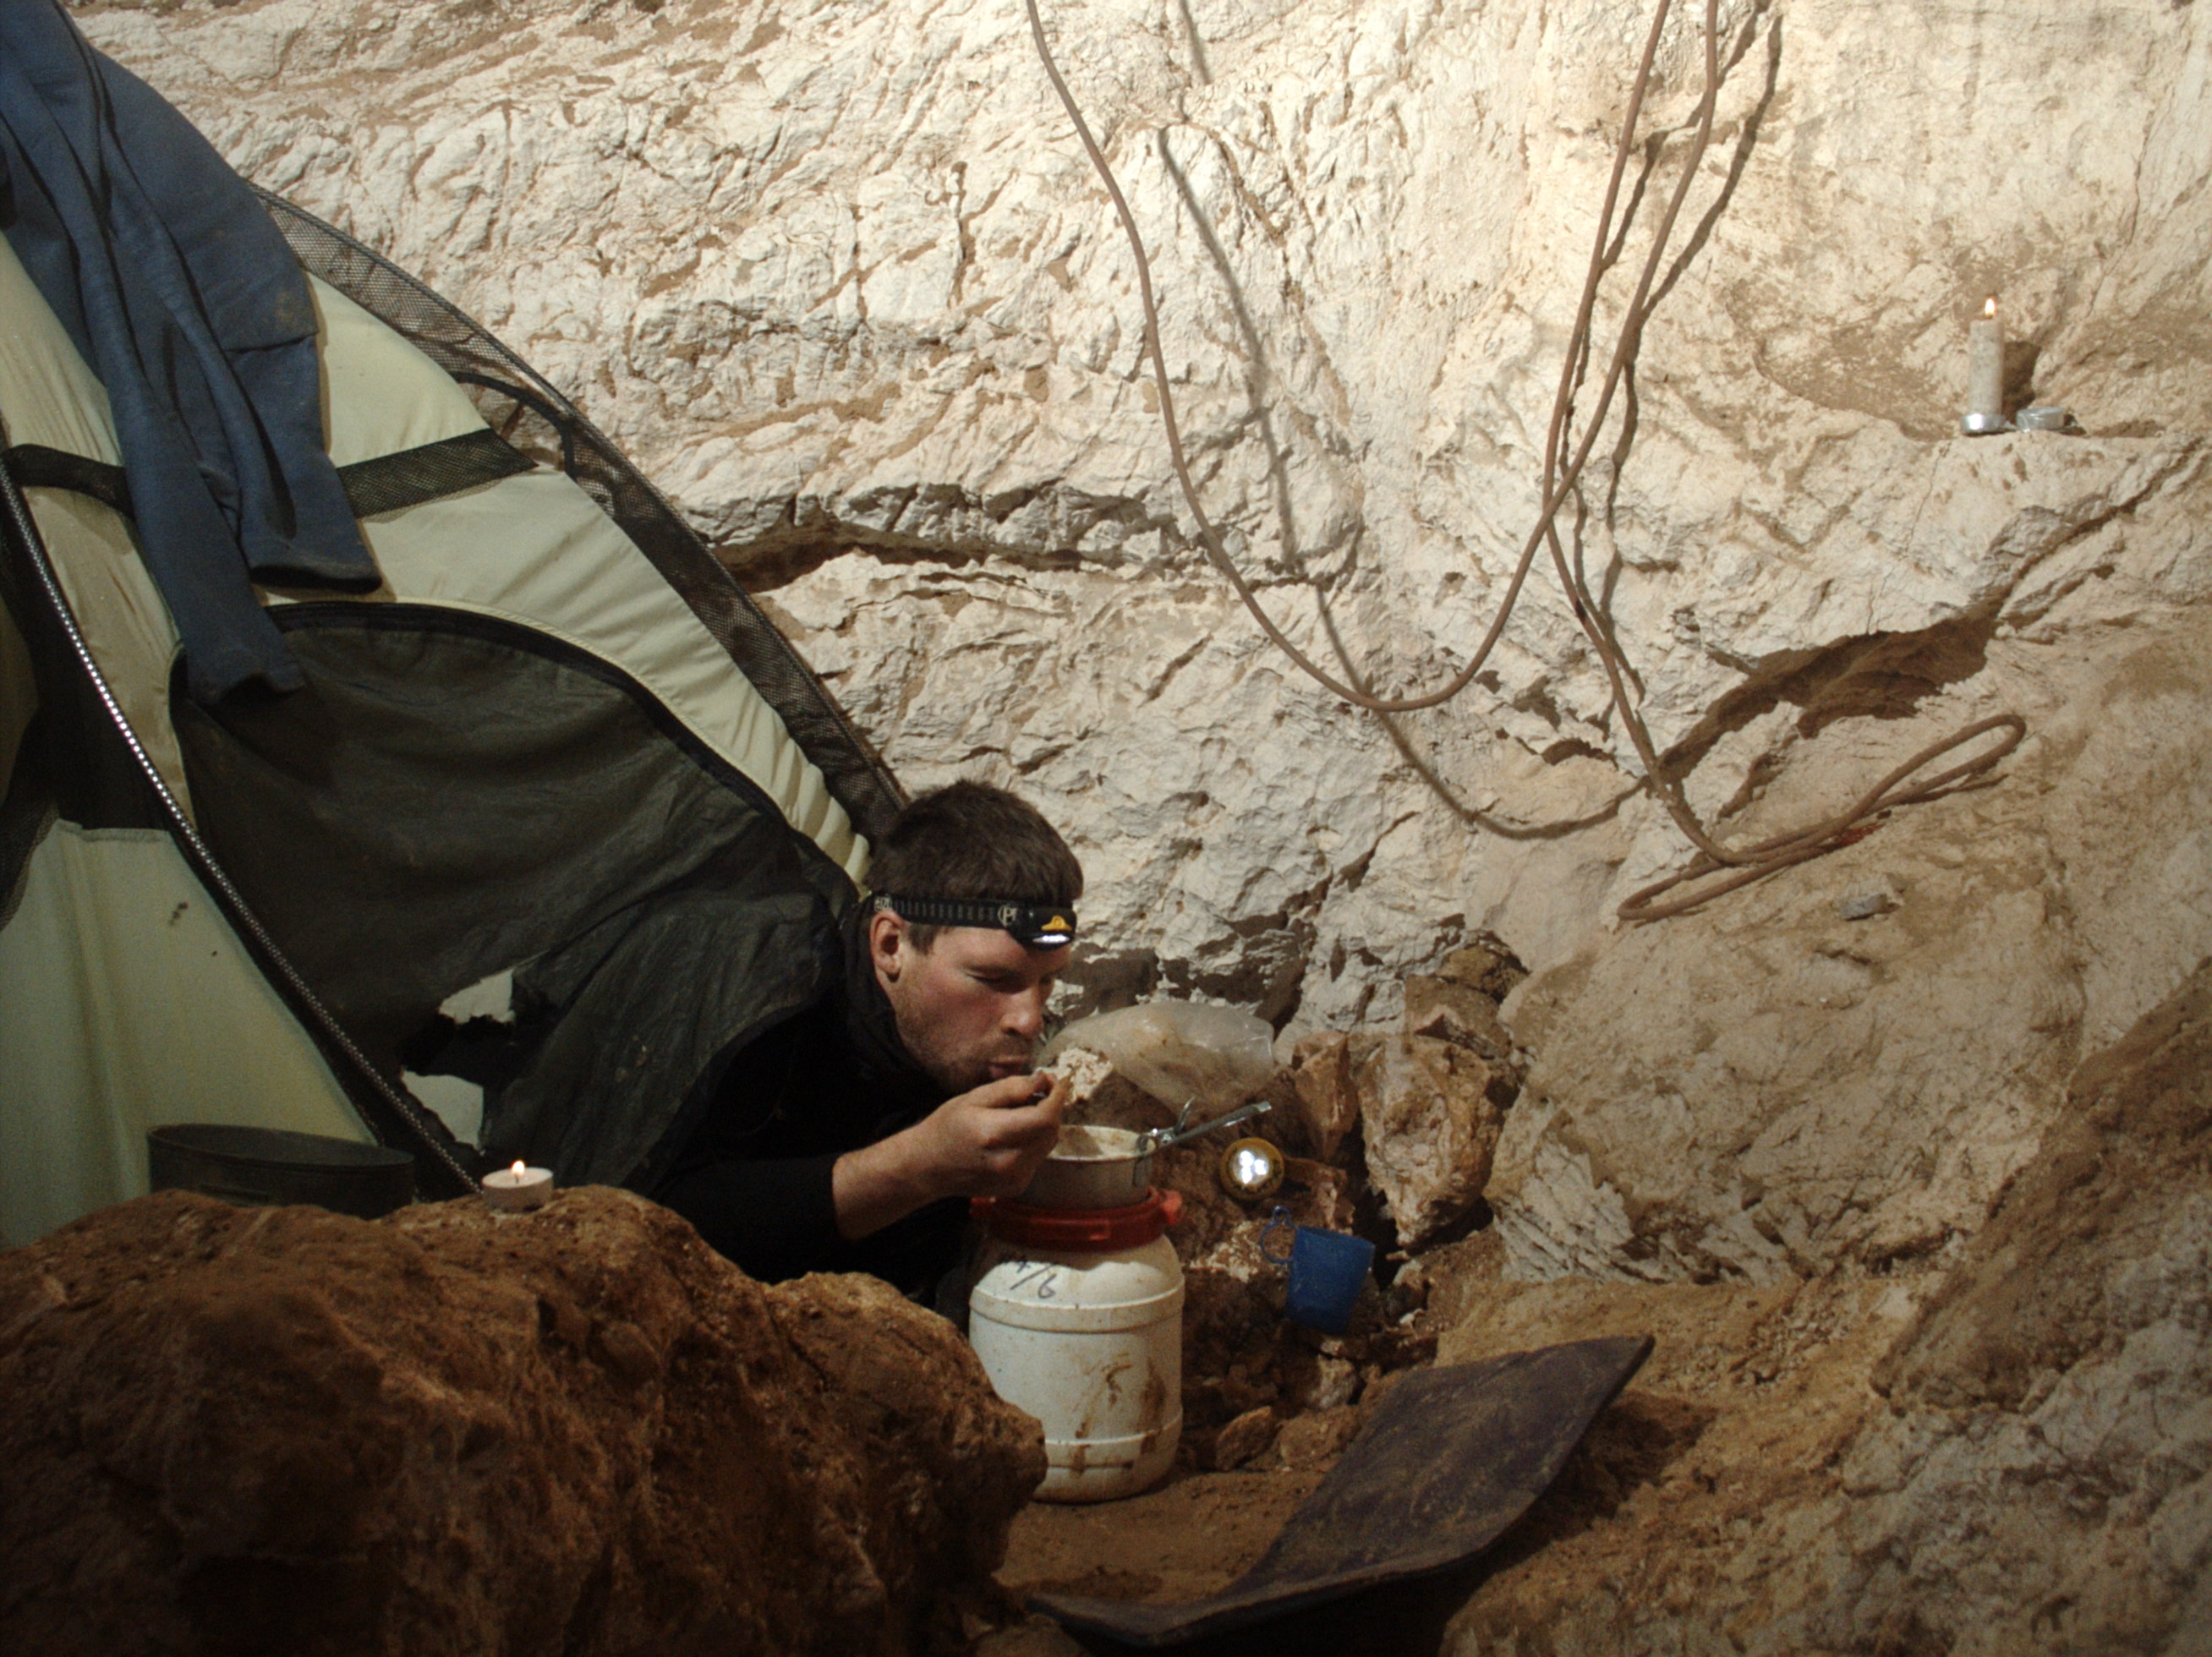
\includegraphics[width=\linewidth]{2009/metal_aven/2009-08-06-11.11.02 - Jarvist Frost - Canon Powershot G5 - Mike eating porridge in the tent--orig.jpg}} 
 \caption{Mike Foley at \passage{Metal Camp}, directly beneath the roped \passage{Metal Aven} climb. \pic{Jarvist Frost}}
 \label{metal aven porridge}
\end{figure*}



We set off for a doss day and decided to climb the 4 m aven on top of
the tent at \passage{Metal camp}. The aven leads to a roomy room (there is
a lead off a side chamber). Izi climbed up to a bolder move - at that
point I scurried down and fetched rope for Izi. I secured a rope to a
sling and I joined him. The next move looked fine. So I roped up (with
the superstatic) and Izi belayed me to a few dubious flakes where the
crurx was! Crux! Exposed move 10 m off the terrace secured by a
superstatic rope and to a very dubious sling. Anyways\ldots{} Another
muddy chamber was reached, pushed to the left to a narrow muddy squeeze
(not really worth digging, I am HO) and a rift to the right which was
pushed to a constriction (lead). Which could be easily bashed --
probably the connection.

\name{James Kirkpatrick}


    \begin{marginfigure}
\checkoddpage \ifoddpage \forcerectofloat \else \forceversofloat \fi
\centering
 \frame{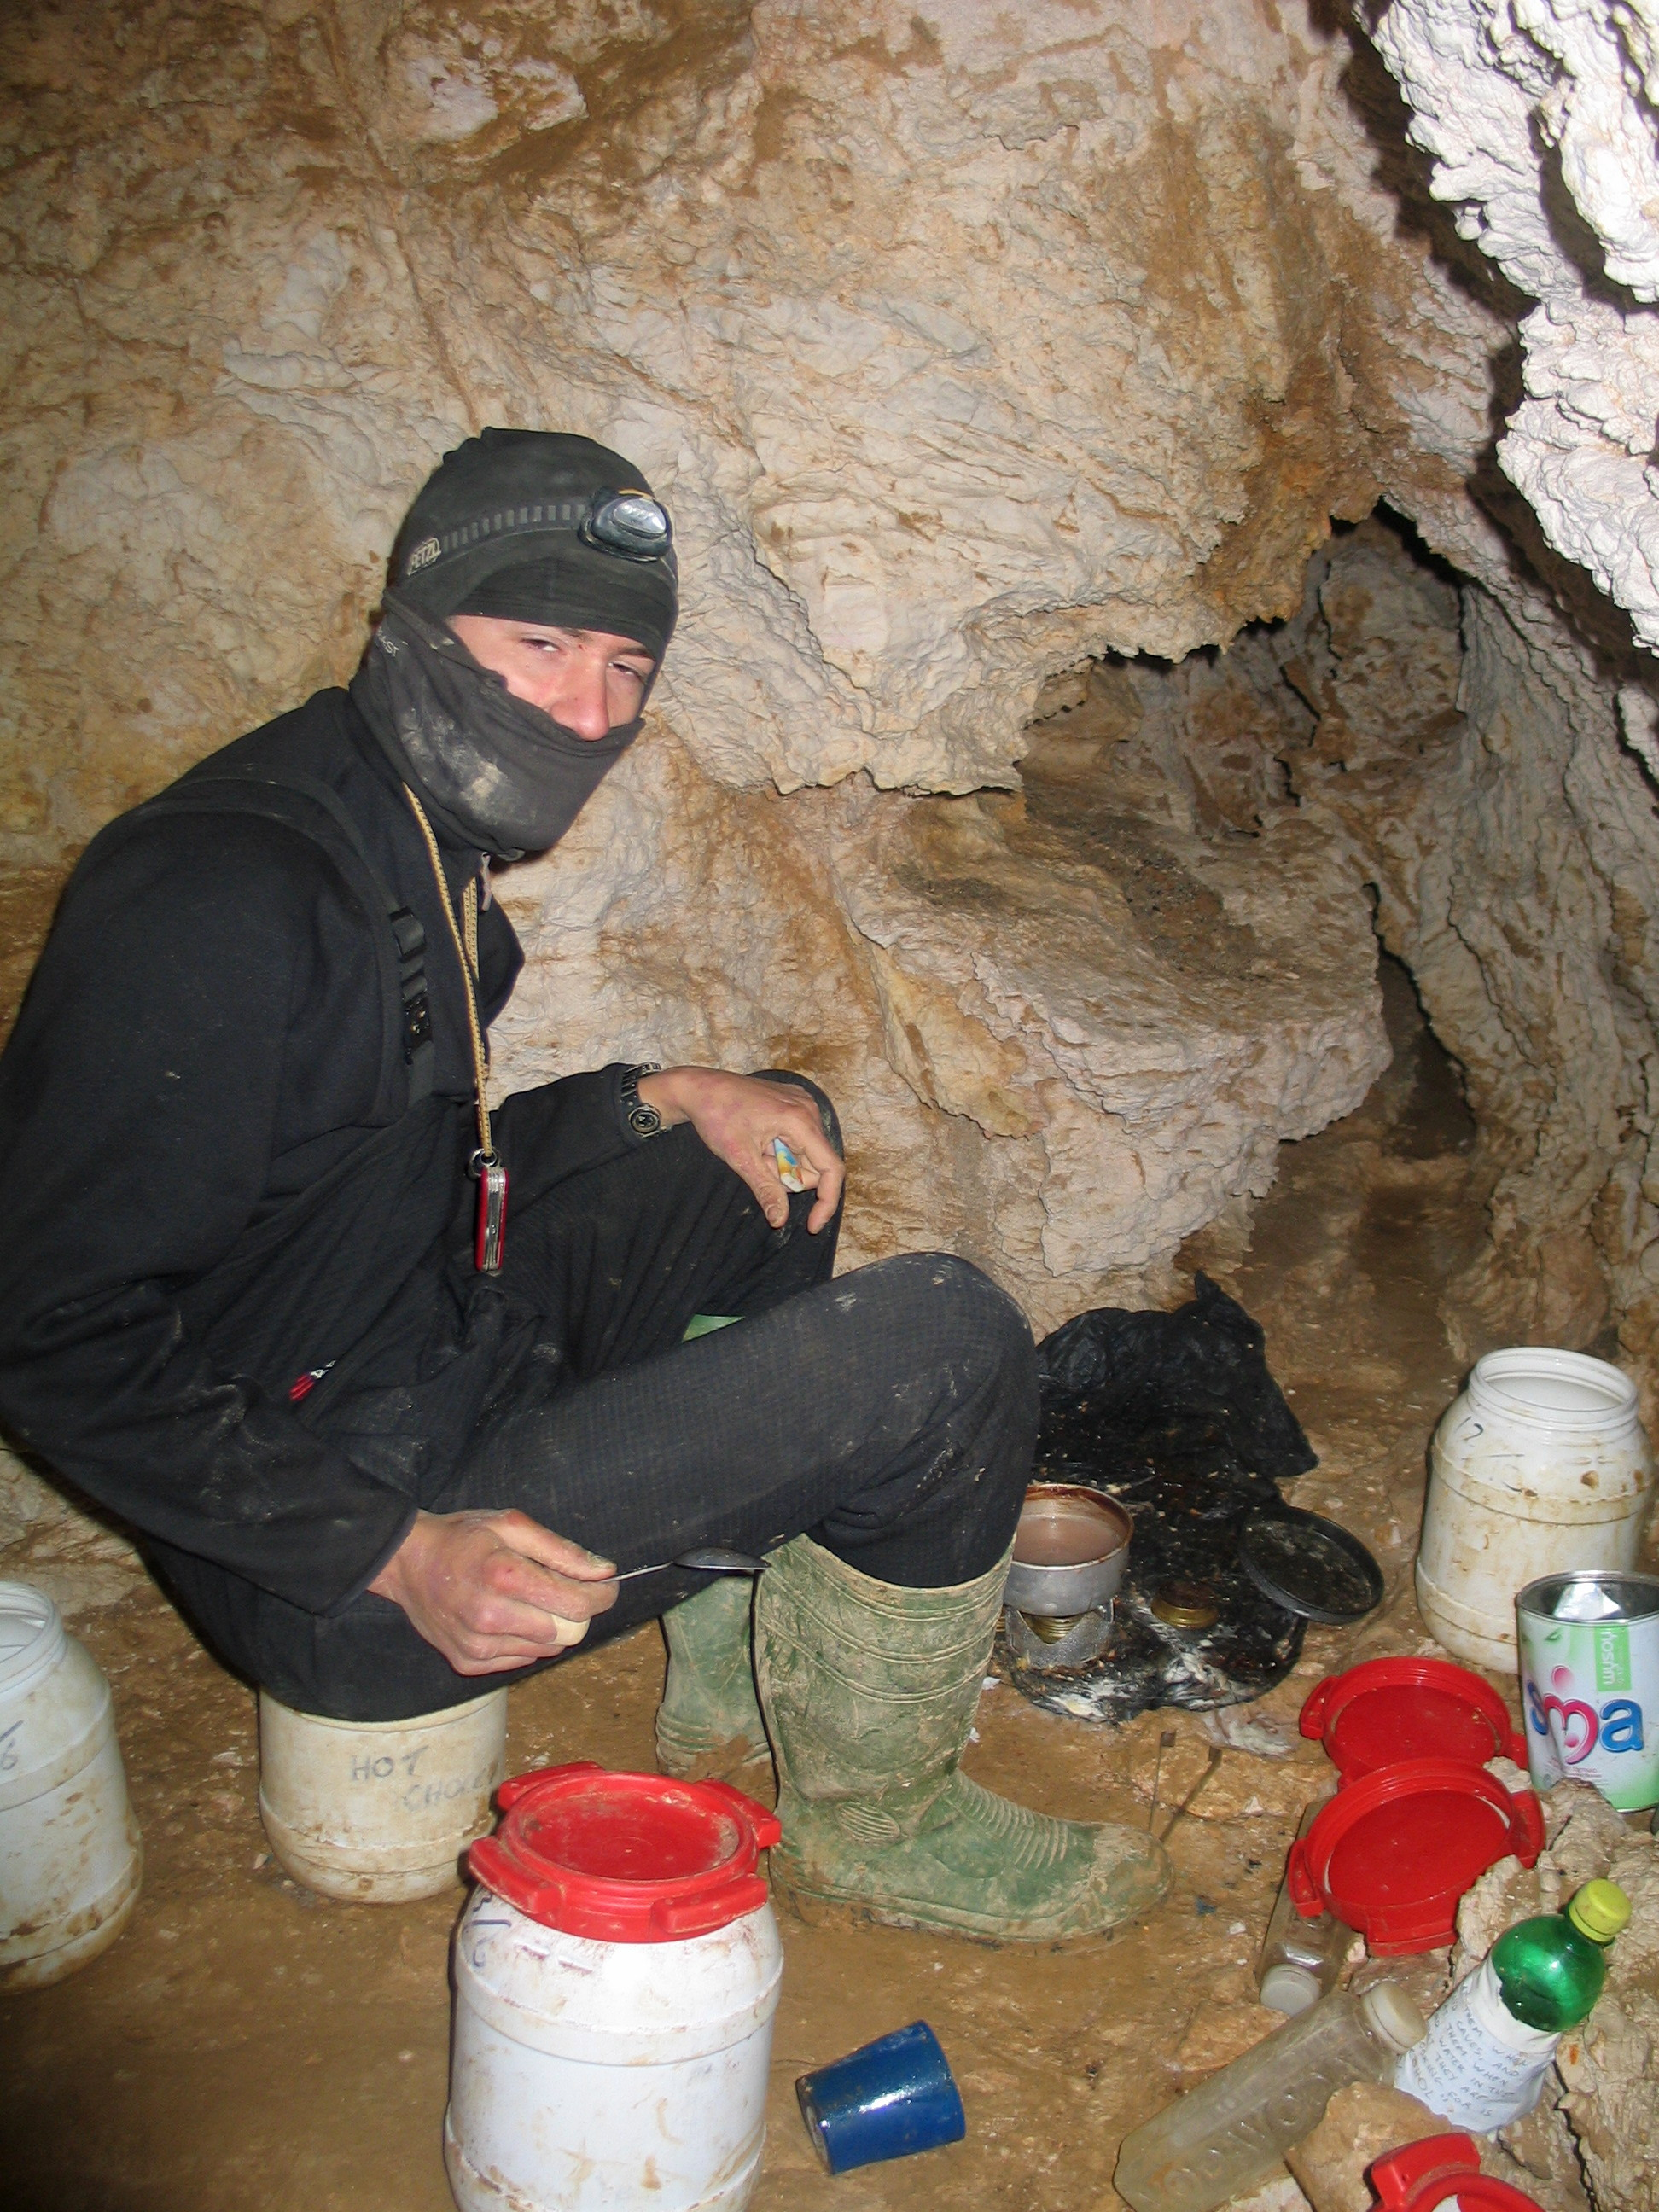
\includegraphics[width=\linewidth]{2009/primula/2009-08-18-10.07.21 - Jarvist Frost - Canon Powershot G5 - Last Camp - Dan cooking--orig.jpg}} 
 \caption{Dan cooking in \passage{Metal Camp}. \pic{Jarvist Frost}}
 \label{metal camp cook}
\end{marginfigure}



\subsection{Climbing \protect\passage{K.E.T.I.}}

\margininbox{K.E.T.I.}{
     \begin{itemize}
    \item Karin Rutar
    \item Erik Bončina
    \item Tjaša Rutar
    \item Izi Možir
    \end{itemize}}{\explo}



The climb in \passage{Primula} did not give me a peace and I really wanted
to do it. I convinced Erik, Tjaša and Karin. For them this was the first
time down \passage{Captain Kangaroo} and I was explaining the stories from previous years.

    \margininbox{Ride the Lightning}{
     \begin{itemize}
     \item Erik Bončina
    \item Izi Možir 
    \item Tjaša Rutar
    \end{itemize}}{\explo}

We quickly arrived to the traverse that James and I were trying to do. First
I tried to go through the boulder choke, and then I send Erik to give it
a go. We decided it is too risky and instead did a climb up to a window
before the choke to bypass it. It was about 4 m to this window and we
could see a rocky spike so we tried to catch it with a lasso. After a
few attempts we made it and Erik went up first and secures the rope
properly. I followed up and after few meters upwards we realised, it
will not bypass the choke but we were curious where it leads. We were
stopped by a very tight squeeze, as none of us could fit through. But we
could see a big chamber through.


\begin{figure*}[t!]
      \checkoddpage \ifoddpage \forcerectofloat \else \forceversofloat \fi
      \centering
    \begin{subfigure}[t]{\textwidth}
    \centering
        \frame{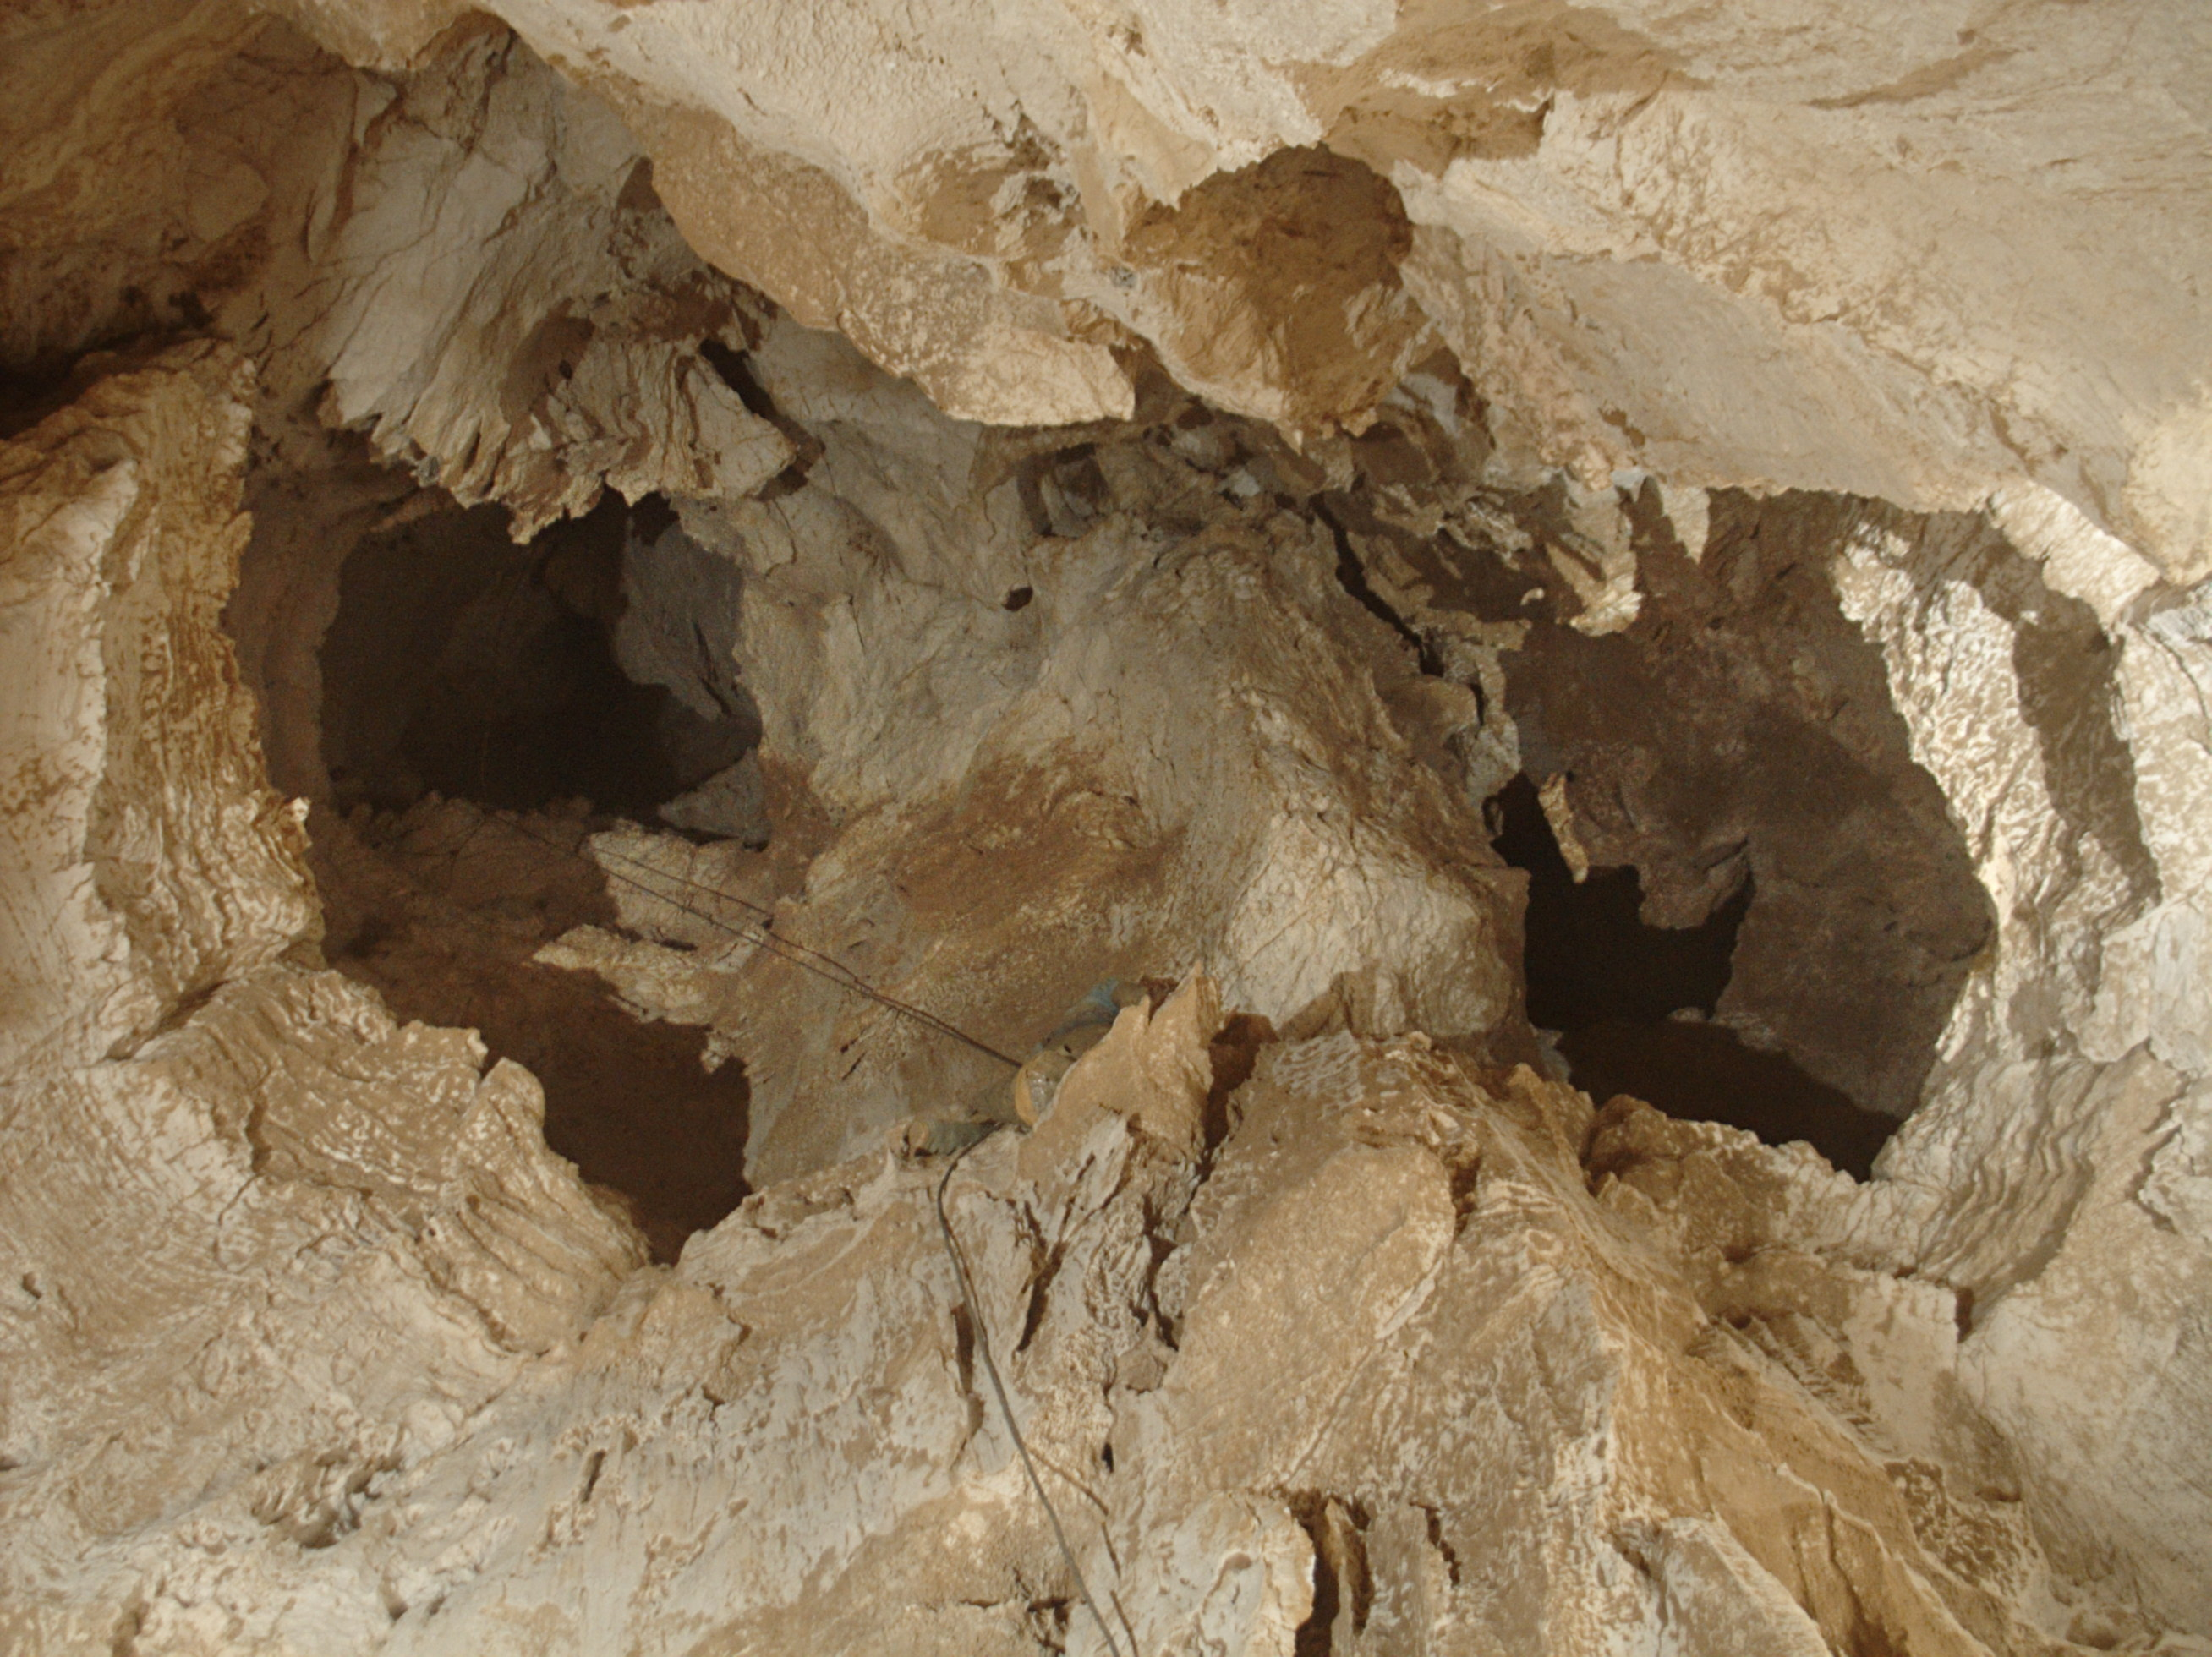
\includegraphics[width=\linewidth]{2009/keti/2009-08-06-13.08.36 - Jarvist Frost - killem all - mike bolting traverse to ride the lightning--orig.jpg}} 
        \caption{} \label{mike bolting to rtl1}
    \end{subfigure}
    
          \vspace{0.3cm}
          
    \begin{subfigure}[t]{0.49\textwidth}
        \centering
        \frame{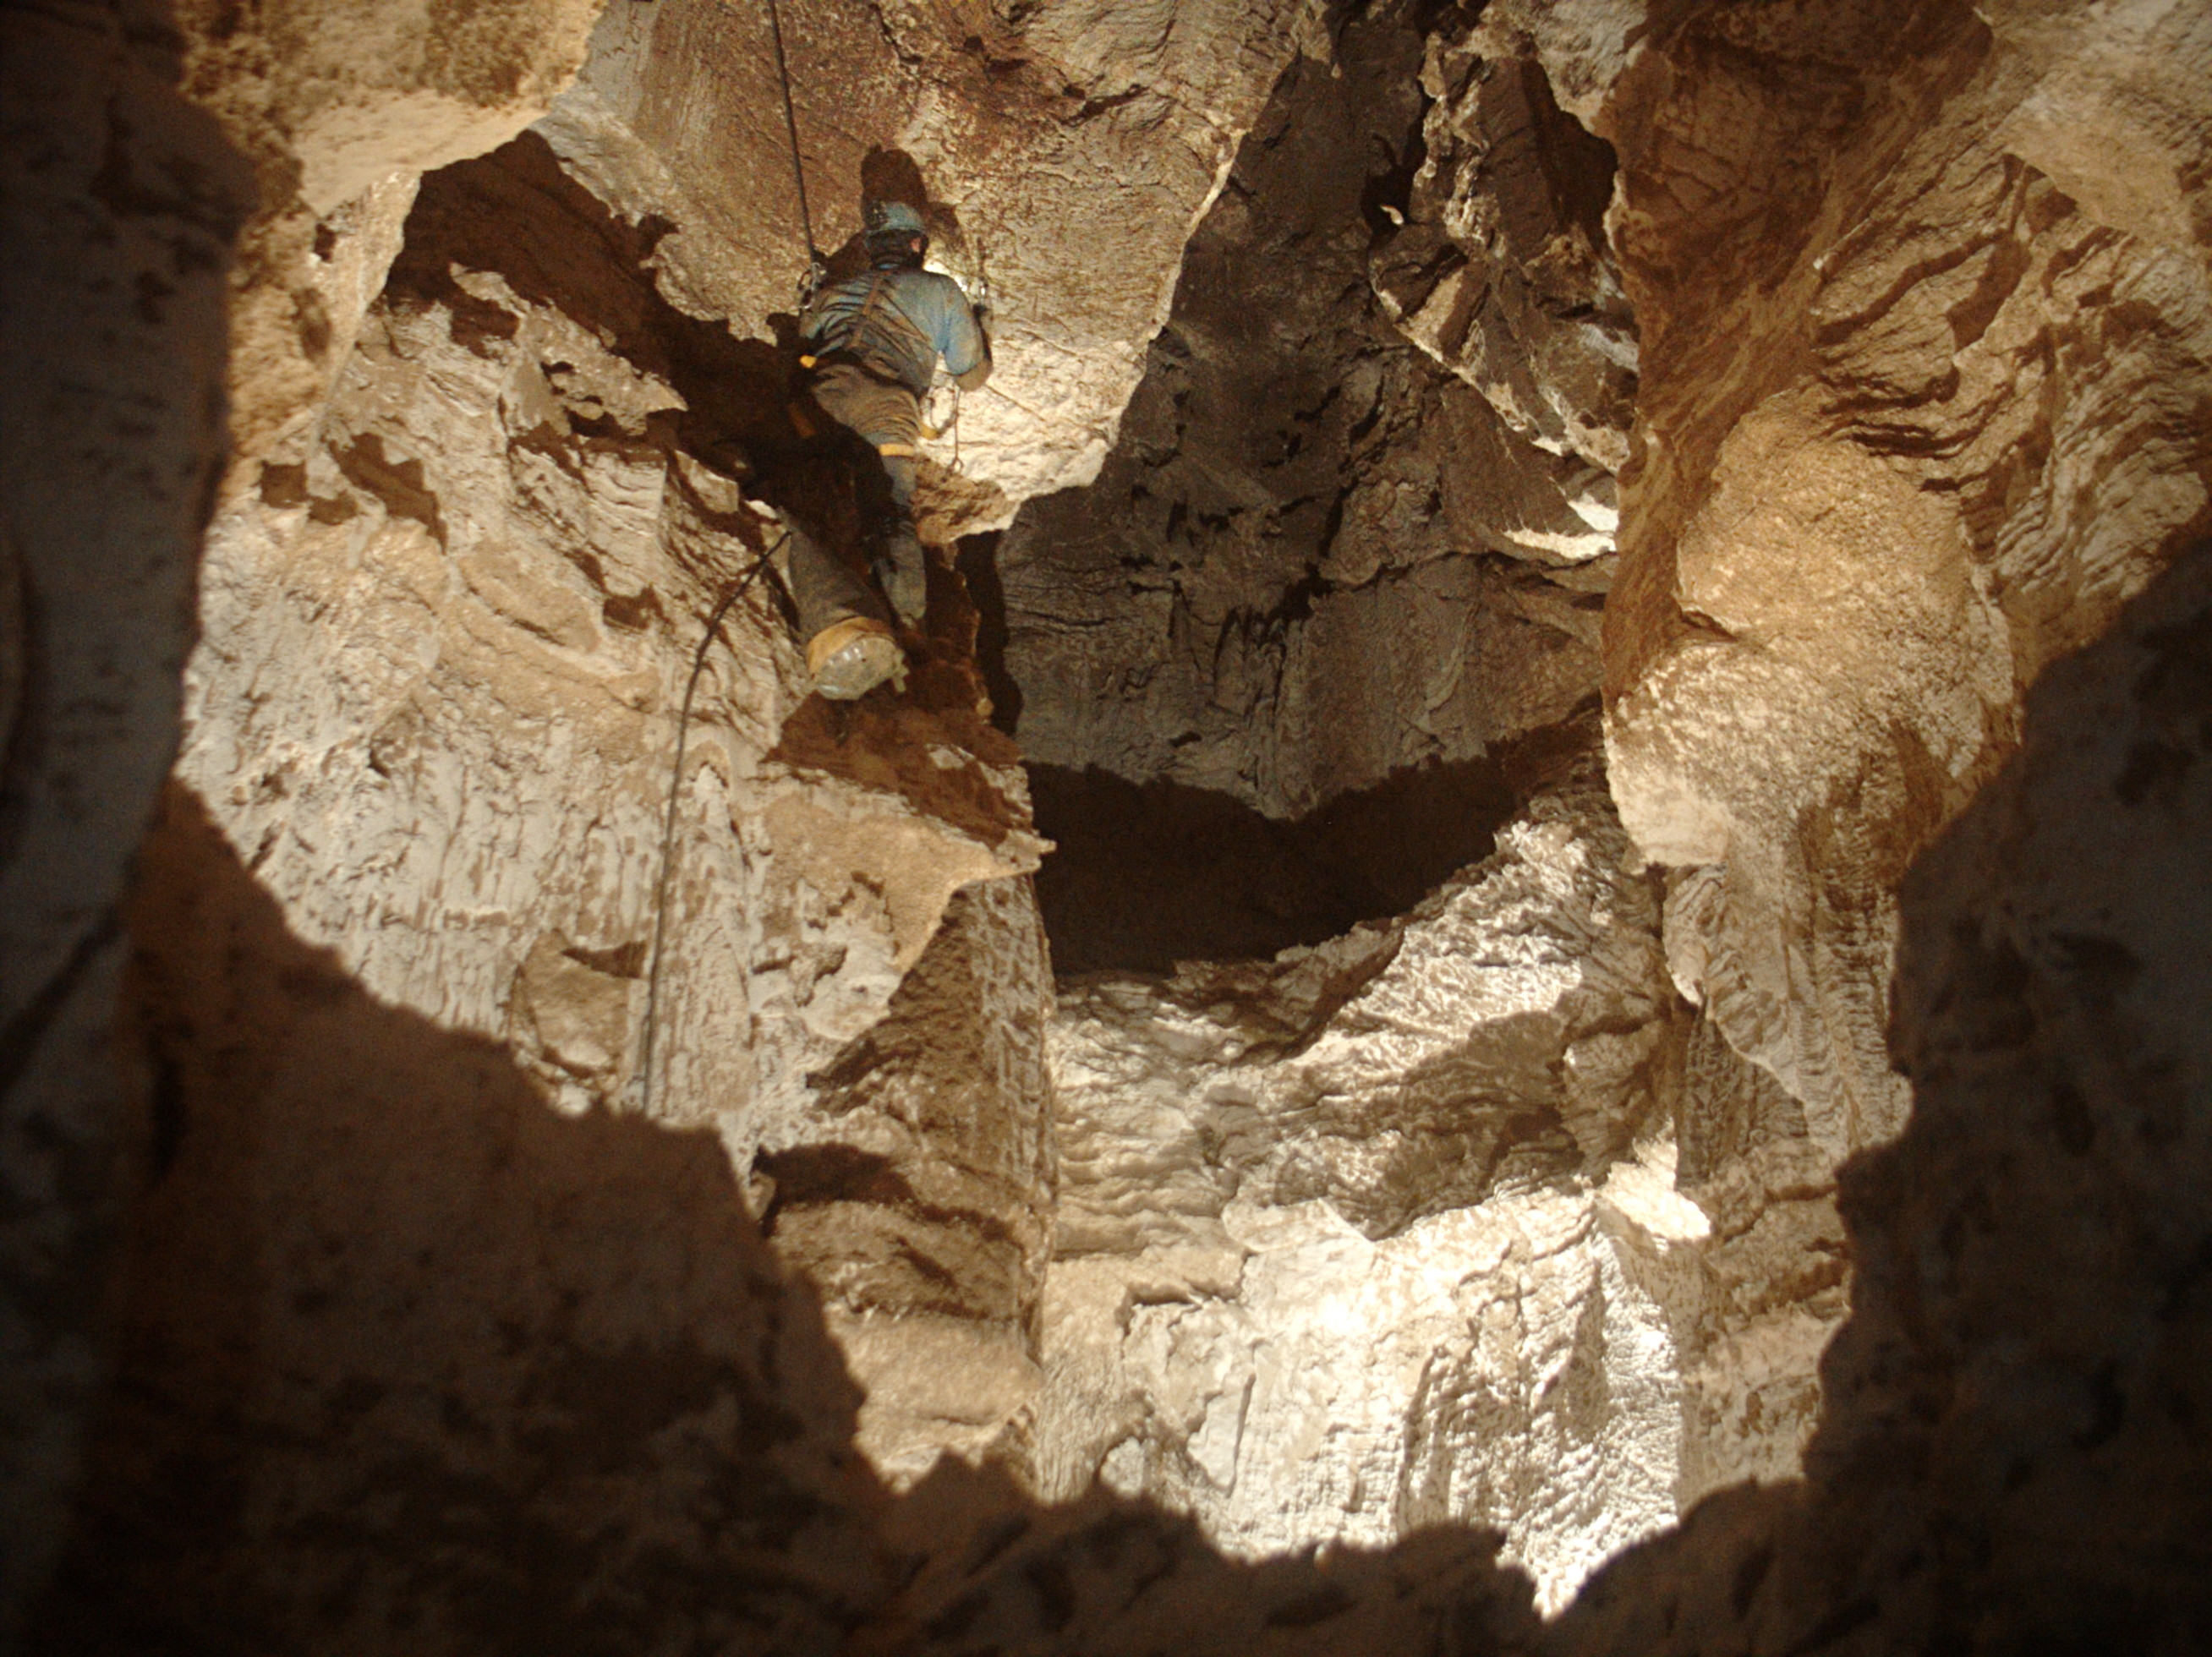
\includegraphics[width=\linewidth]{2009/keti/2009-08-06-13.11.30 - Jarvist Frost - killem all - mike bolting traverse to ride the lightning view from intravenus window--orig.jpg}} 
        \caption{} \label{mike bolting to rtl2}
    \end{subfigure}
    \hfill
    \begin{subfigure}[t]{0.49\textwidth}
        \centering
        \frame{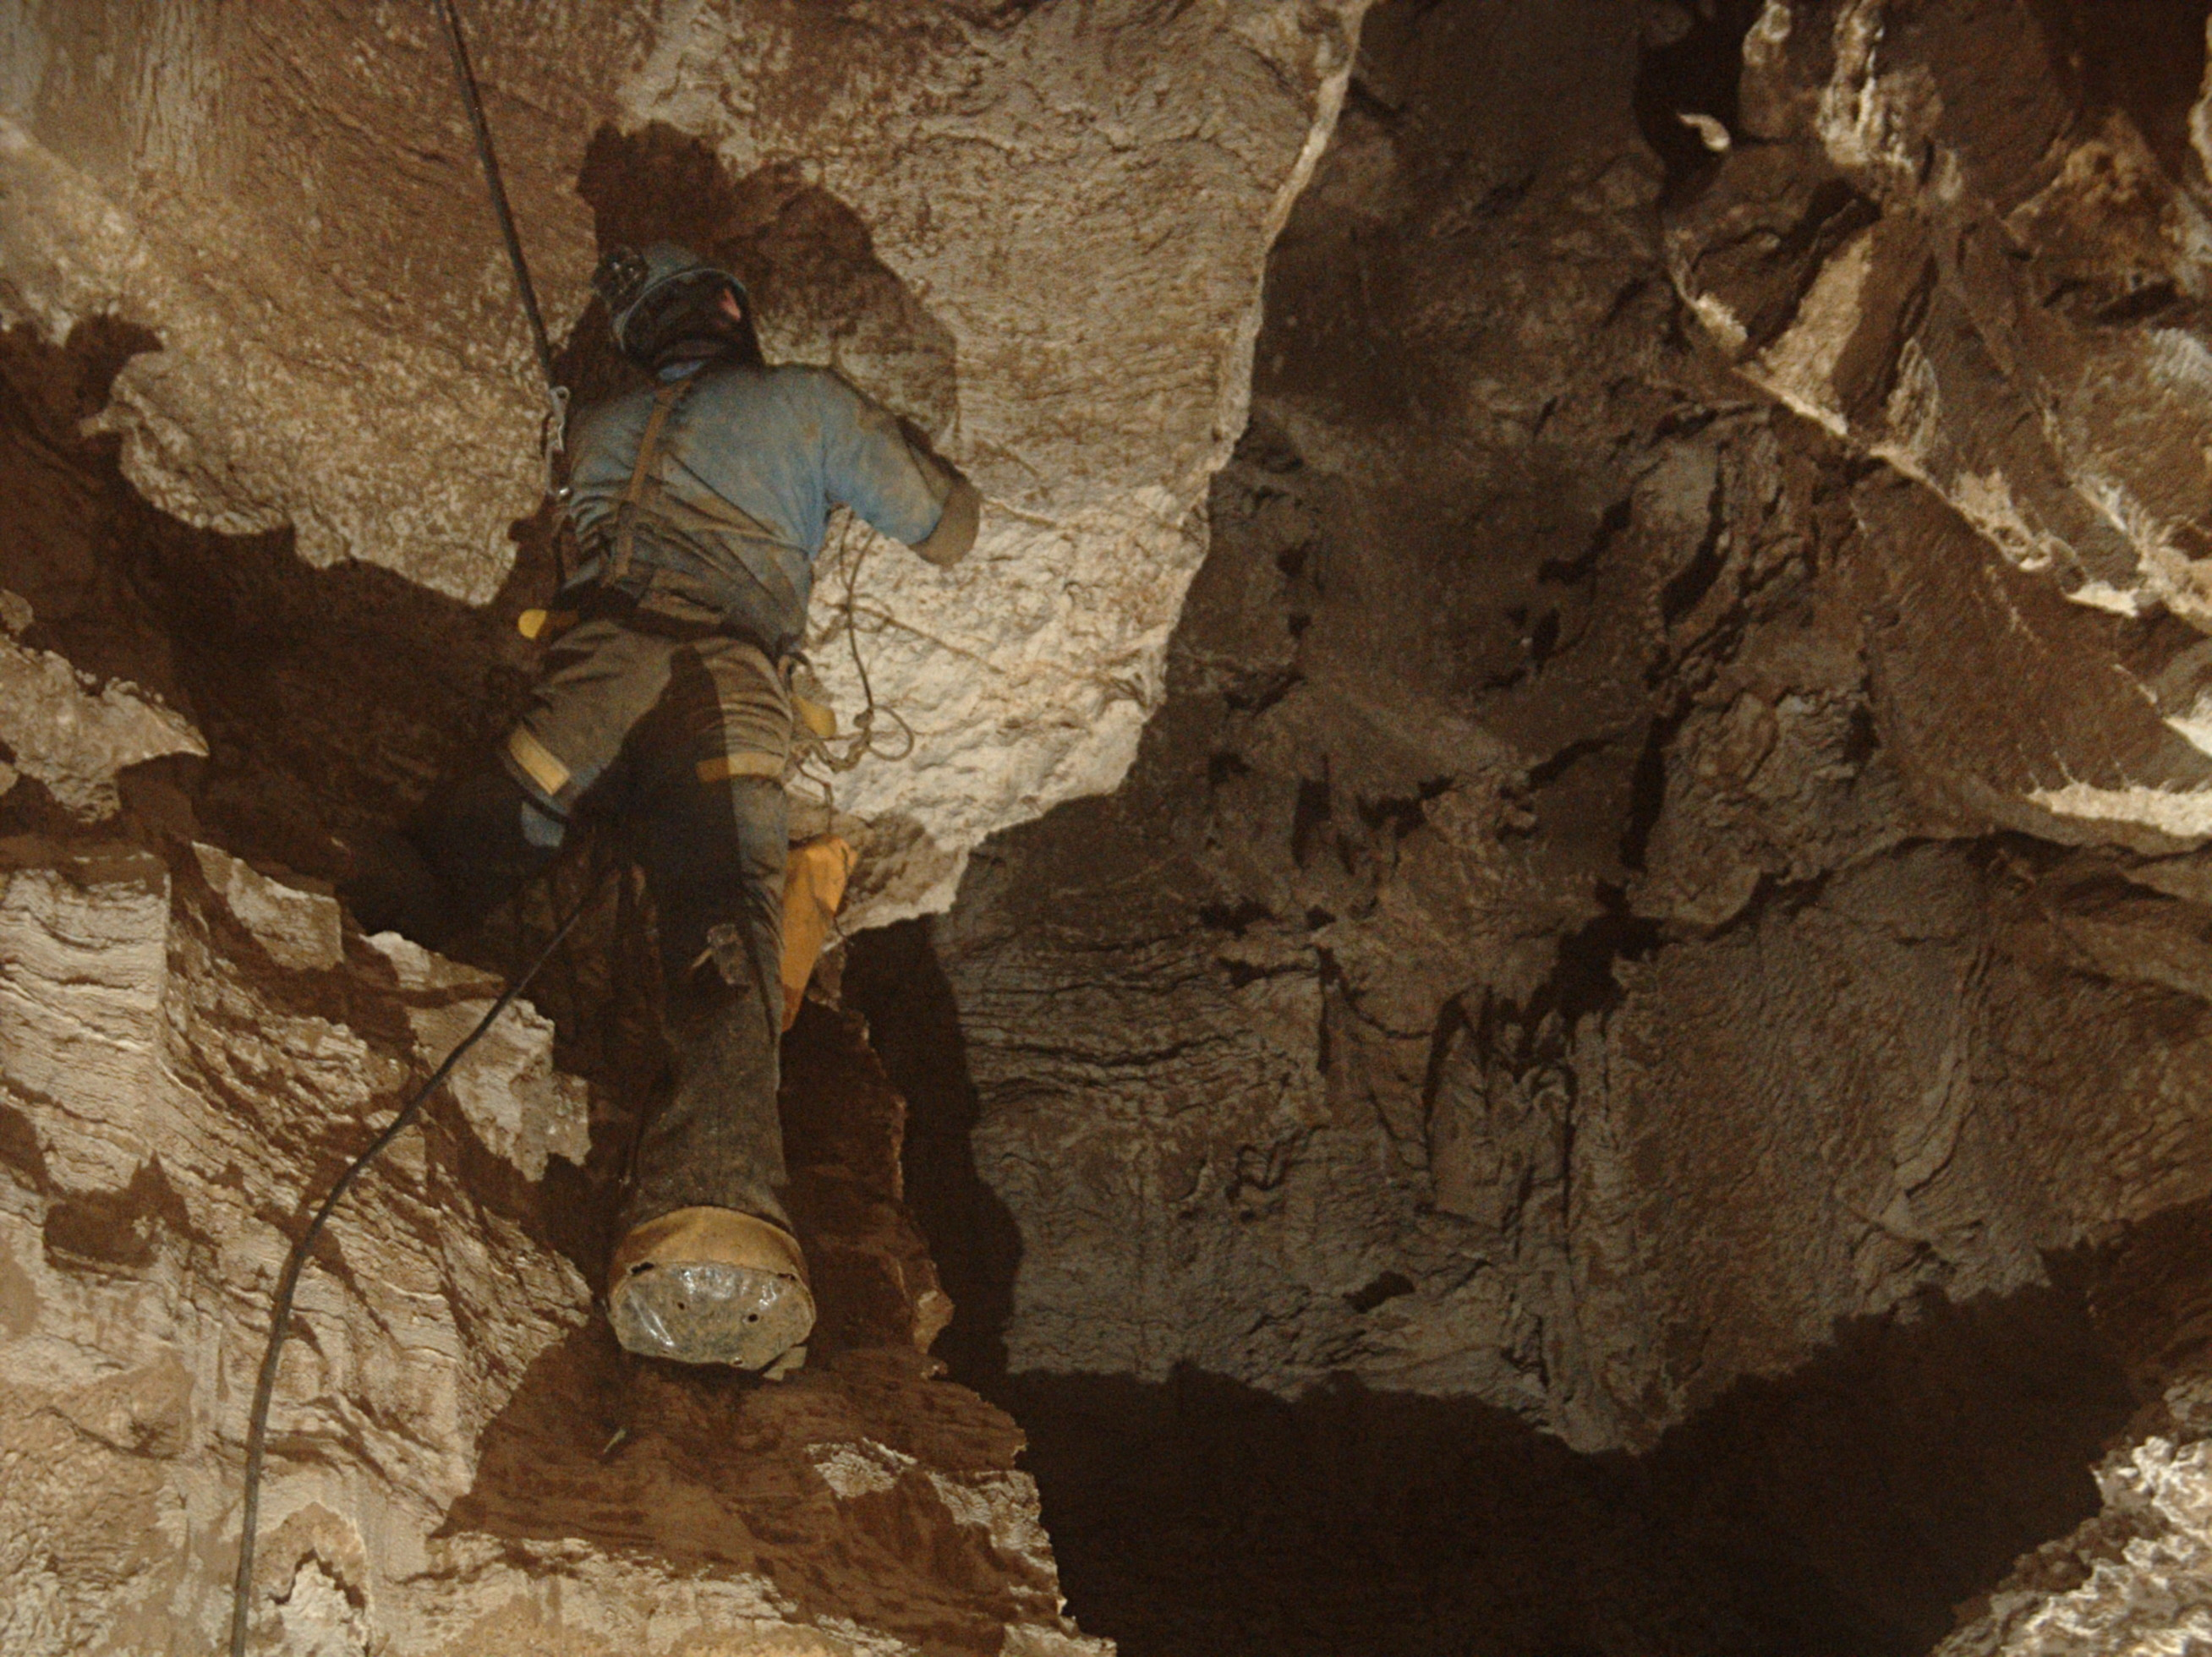
\includegraphics[width=\linewidth]{2009/keti/2009-08-06-13.12.44 - Jarvist Frost - killem all - mike bolting traverse to ride the lightning view from intravenus window2--orig.jpg}} 
        \caption{} \label{mike bolting to rtl3}
    \end{subfigure}

    \caption{Mike Foley bolting a traverse across \passage{Kill'em All} towards the ledge below \passage{Ride the Lightning} on 6th August. \pic{Jarvist Frost}
    }
\end{figure*}

We decided to throw a note with the
name \passage{K.E.T.I.} written on it, so if anyone will arrive to this chamber they will know that \passage{Primula} is on the other side. At this point we heard the voices and started shouting. It was Thara and Tim. We asked
them, if they can see the note and where exactly are they. After
laughing, they said they are in \passage{Metal camp}. That tells us, that
there is another way to \passage{Primula} without going through
\passage{Kill'em All} pitch. We surveyed back to \passage{Primula}.

\name{Izi Možir}


\subsection{Climbing \protect\passage{Ride The Lightning}}

After \passage{Primula} mission we still had time, so we decided to check
out Jarv's lead in ``\passage{Kill'Em All}''.

In the middle of the \passage{Kill'em All} pitch Jarv made a traverse to a
ledge. Here is a climb, so we decided to give it a go. This ledge is
small and just about fitted all 4 of us.

I decided to try the climb first. I attached the rope to myself and
started climbing. Meanwhile Erik was connected to that rope in case I
would fell on the ledge but miss it and start falling down the pitch. On
the top I bolted and use a natural for a backup. From here I could see a
pitch and others came up as well. We did not have enough rope to reach
the bottom so we left it undescended. We named this climb \passage{Ride the
Lightning}.

\name{Izi Možir}


\newpage
\begin{pagefigure}
\checkoddpage \ifoddpage \forcerectofloat \else \forceversofloat \fi
\frame{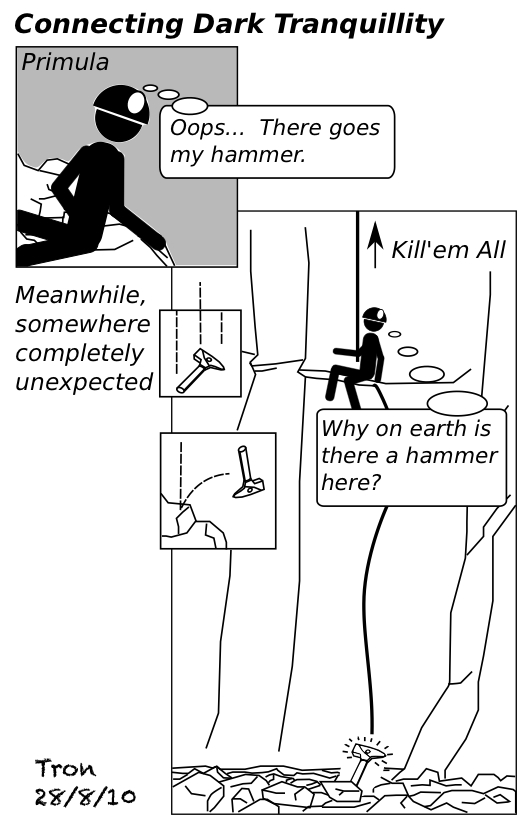
\includegraphics[width=\linewidth]{2009/logbook/Tharatorn Supasiti - March 2012 - dark-tranquillity--orig.jpg}}
\caption{Interconnected cave passages might lead to surprises. \pen{Tharatorn Supasiti}} \label{DQ cartoon}
\end{pagefigure}
